\begin{figure}[H]
    \centering
    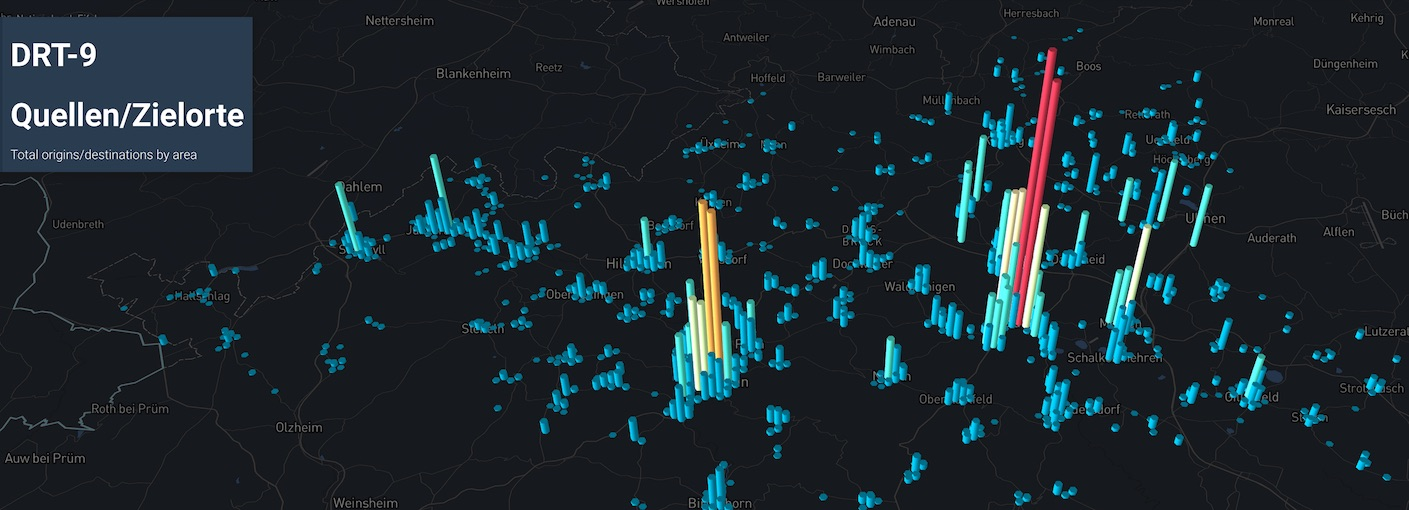
\includegraphics[width=0.8\textwidth]{assets/xy-hexagons.jpg}
    \caption{Origin/Destination point data aggregated into hexagons}
\end{figure}

Counts the number of points that occur inside hexagons of arbitrary size.

\hypertarget{usage}{%
\subsection{Usage}\label{usage}}

A file named \texttt{viz-xy-*.yml} will match and trigger the creation
of the XY hexagon plot.

In addition, the presence of the MATSim regular output file
\texttt{output-trips.xml.gz} will automatically trigger an XY Hexagon
plot depicting the trip origins and destinations present in that file.

\hypertarget{dashboards}{%
\subsection{Dashboards}\label{dashboards}}

XY Hexagon plots can be embedded in dashboards using
\texttt{type:\ hexagons} and specifying the config details in the props
as follows:

\begin{lstlisting}
row:
- title: My Hexagon Plot
    type: hexagons
    # ...
\end{lstlisting}

\hypertarget{yaml-fields-explained}{%
\subsection{YAML fields explained}}

\textbf{title:} (optional) title of the visualization, appears right on
top of the map. If a title is specified both under ´general´ and under
´props´, the one under ´general´ will be used.

\textbf{description:} (optional) description of the visualization,
appears between title and map. If a description is specified both under
´general´ and under ´props´, the one under ´general´ will be used.

\textbf{file:} a csv, json or gzip'ed json file containing an array with
the data.

\textbf{projection:} EPSG code of the projection

\textbf{elements:} the name of the property containing the data array
(for JSON files only)

\textbf{thumbnail:} (optional) file path to a thumbnail in jpg format

\textbf{center:} (optional) coordinates that the map centers on. Can be
provided as array or string. If it is not provided, a center is
calculated using a sampling of the data.

\textbf{zoom:} (optional) zoom level of the map between 5 and 20. If it
is not provided, the zoom level 9 is used.

\textbf{radius:} starting radius of the hexagons.

\textbf{maxHeight:} (optional) starting height of the hexagons. If it is
not provided, 0 is used.

\textbf{aggregations:} a list of \texttt{title}, \texttt{x}, \texttt{y}
which say which columns of data in the elements array contain the x,y
data. x,y can be column numbers or column names. You can specify
multiple aggregations in the data section. \emph{Note: column numbers
are zero-based!}

\hypertarget{xy-data-file-format}{%
\subsection{XY Data File format}\label{xy-data-file-format}}

JSON and CSV files are supported.

\textbf{CSV:} a simple CSV with a header column is all that's needed.

\textbf{JSON}: The file must have an object with a property whose name
is the element. Here's an example that matches the sample YML above.

In this example, each array element is also an array with xy data in
columns 0,1 and 3,4. The row elements can also be regular JSON objects,
in which case the x/y columns can be referenced by name instead number.

\begin{lstlisting}
{
    "drtRequests": [
        [ 6.2343, 52.123, 0, 6.33, 52.23, 0],
        [ 7.0341, 51.237, 0, 7.81, 51.44, 0],
        ...
    ]
}
\end{lstlisting}

All other elements in the JSON are ignored.

\hypertarget{example-yaml-configs}{%
\subsection{Example YAML configs}\label{example-yaml-configs}}

\textbf{viz-xy-example.yml}

\begin{lstlisting}
title: 'XY Example-1: DRT Vehicles'
description: 'Total origins/destinations by area'
file: drt-vehicles.json.gz
thumbnail: thumbnail-vehicles.jpg
center: [6.9814, 51.57]
zoom: 10
radius: 200
maxHeight: 30
elements: drtRequests # only if json
aggregations:
    OD Summary:
    - title: Origins
        x: fromX
        y: fromY
    - title: Destinations
        x: toX
        y: toY
    Base Runs:
    - title: Origins
        x: baseFromX
        y: baseFromY
    - title: Destinations
        x: baseToX
        y: baseToY
\end{lstlisting}

